\chapter{関連研究}

\section{Gated context CNN}
Gated context CNN (以下GTCNN) は, 図\ref{fig:GTCNN_overall}に示すように入力層, 出力層, 中間層である$L$個のGCBR層(Gated CBR Layer)からなる. GCBR層はノイズ除去のみを行うCNN (CBR) とコンテクスト抽出のみを行うCNN (GTL) とに分離されている. GTLが抽出したコンテクストはgate機構を介してCBRに渡されノイズ除去を制御する. このように機能分離を行うことで, 機能分離を行わない既存手法と比較して高いノイズ除去性能を獲得でき, またパラメータ数の削減に成功した. 


\subsection{GTL}
GTLはマルチスケール構造のU-Net\cite{U-net}をベースに設計されている. 一般的なU-Netのエンコーダは$S$段の層を持ち, その階層が下がるたびに特徴量のスケールを半減させ, チャンネル数を倍増させる. デコーダはエンコーダと同数の$S$段の層を持ち, 階層が上がるたびに特徴量のスケールを倍増させ, チャンネル数を半減させる. エンコーダ側では段階的にスケールのサイズが半減するため, CNNのカーネルのサイズが一定でも受容野の広さが倍に増大し, これによって広くコンテクストを把握できるようになる. 一方で, チャンネル数を倍増させることが計算コストの増大にもつながる. GTLでは, 階層を下げるときにチャンネル数を増やさないように変更を加えることで計算効率を高めている. 一般的なU-Netを用いたノイズ除去とはことなり, GTCNNのGTLはコンテクストの把握のみに注力できる(ノイズ除去はCBR層が行っている)ため, チャンネル数を増加させずとも良い性能が得られていると推測されている. 


\begin{figure}[ht]
\centering
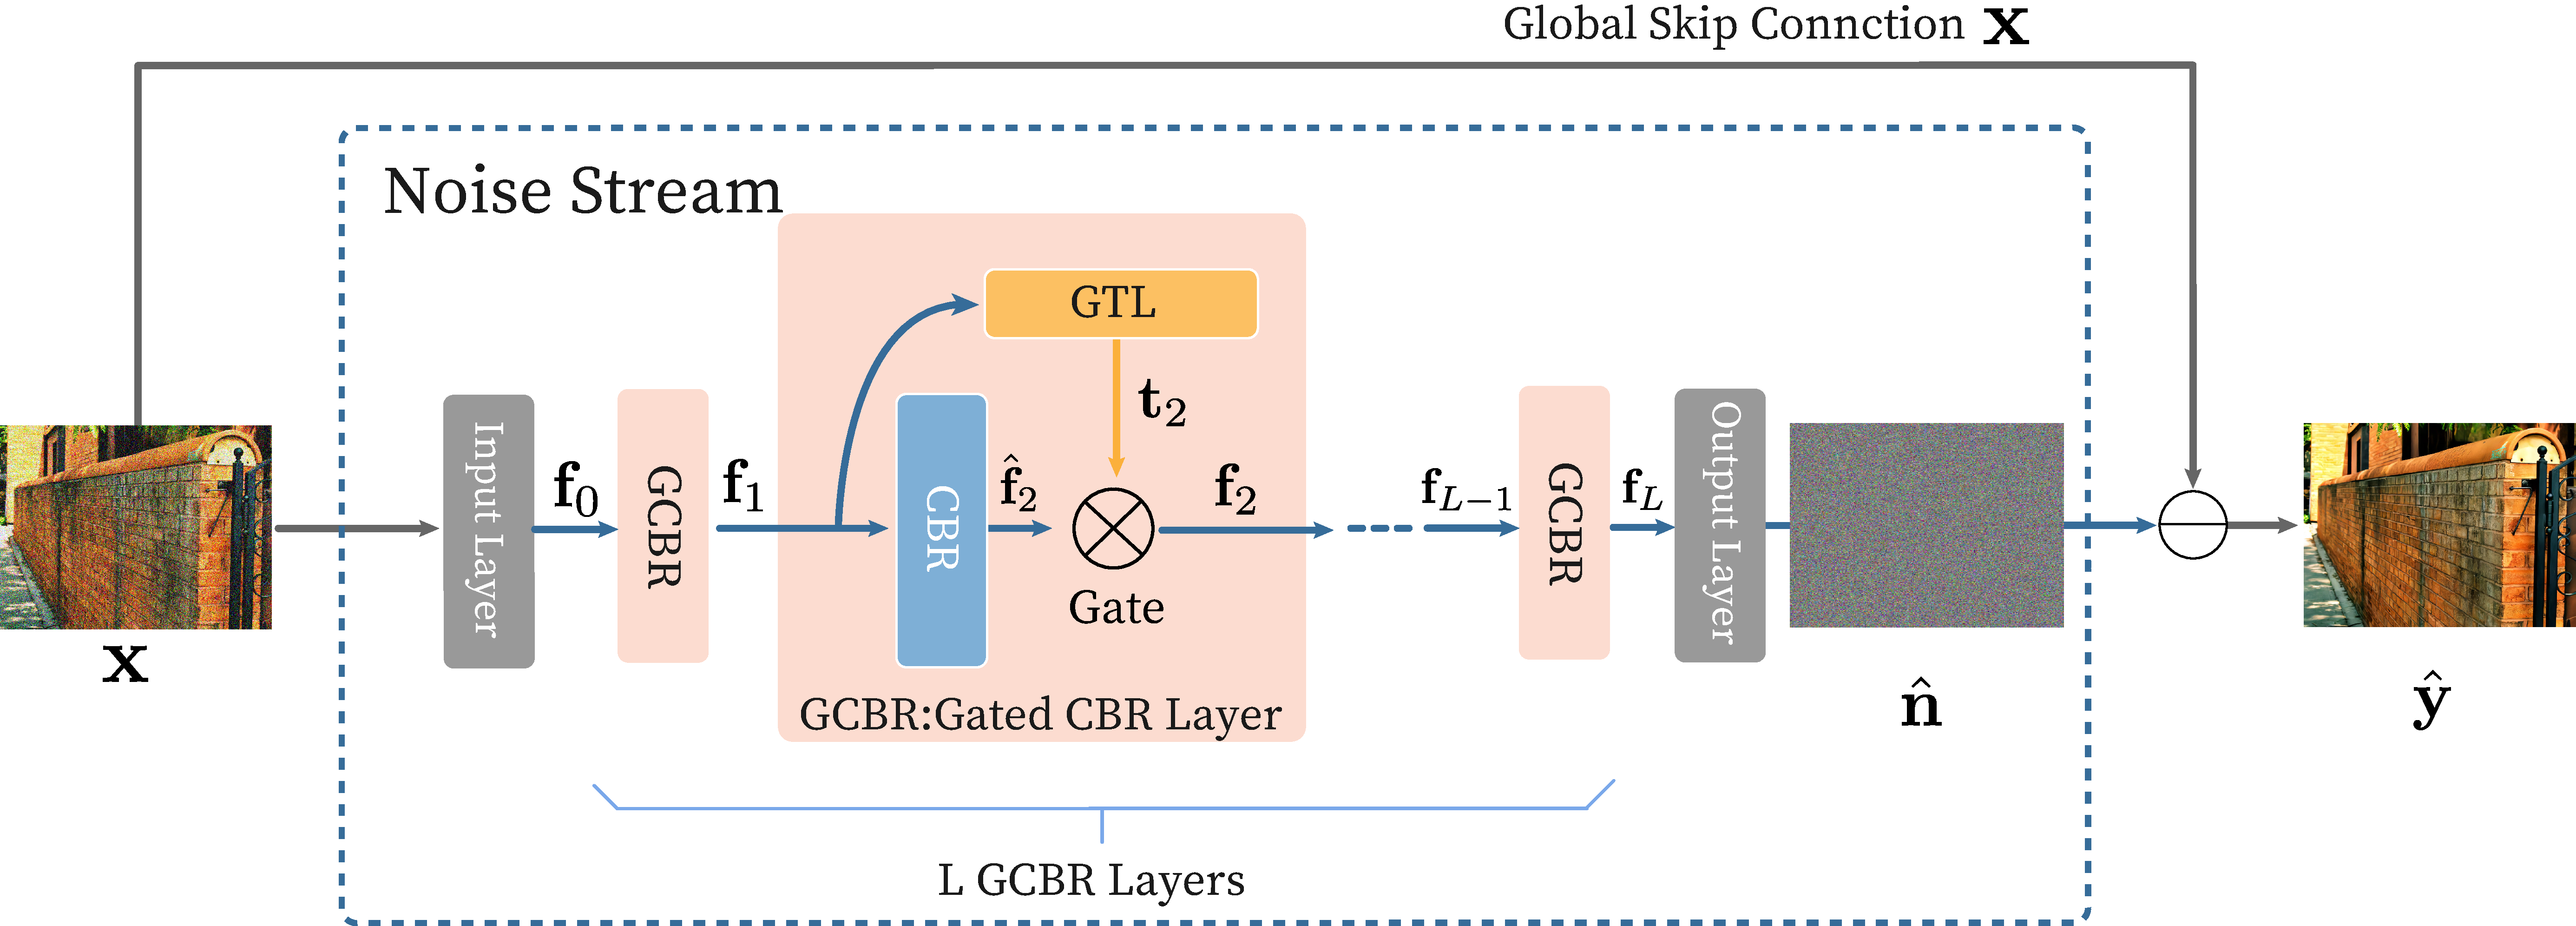
\includegraphics[scale=0.13]{figures/GTCNN_overall.pdf}
\caption{GTCNNのアーキテクチャ全体図. 文献\cite{GTCNN}より引用. (C) 2020 Springer \label{fig:GTCNN_overall}}
\end{figure}

\section{Vition Transformer}
Vision Transformer (ViT) \cite{ViT}は自然言語処理の分野で用いられていたTransformerを画像処理の分野で活用可能なものにし, また画像分類タスクの性能を向上をさせた手法である. それまで画像処理タスクはCNNに大きく依存しており, またCNNはその性質上広域なコンテクストの取得が難しかった.\\
 ViTは画像を複数のパッチの集合とすることで自己注意主体のネットワーク構造で画像を処理することが可能となった. パッチをトークンに見立て, それに一般的なTransformer同様に埋め込み処理を行いそれをTransformerのEncoderに入力する. そして出力されたデータをMLPを通しクラスデータを抽出する.\\
 図\ref{fig:vit_overall}のTransformer Encoder部を式で記述すると以下のようになる. Transformer Encoderにはパッチに埋め込み処理を施されたデータ$\bm{z}_{0}$が初めに入力される.
 \begin{align}
\bm{z}^{\prime}_{l} &= MSA(LN(\bm{z}_{l-1})) +\bm{z}_{l-1},& &l = 1 \cdots L \\
\bm{z}_l &= MLP(LN(\bm{z}^{\prime}_{l})) + \bm{z}^{\prime}_{l},& &l = 1 \cdots L
 \end{align}

$LN$はレイヤーノルム, $MLP$は多層パーセプトロン, $MSA$が自己注意を表している. 自己注意は式(\ref{eq:SA})のように表される\cite{SA}. $\mathbf{Q,K,V}$は入力にそれぞれ異なる埋め込み処理をしたものである.
\begin{align}
Attention(\mathbf Q,\;\mathbf K,\; \mathbf V)=softmax(\frac{\mathbf Q \mathbf K^T}{\sqrt{d_k}})\mathbf V \label{eq:SA}
\end{align}
 式(\ref{eq:SA})では$\mathbf{Q}$と$\mathbf{K}$から得られる全データ間の類似度をもとに, $\mathbf{V}$を処理することを表しており, このことから, 局所的な処理をするCNNとは異なり, 自己注意は大域的な処理を行っているということである. ViTではこの特性のため広域なコンテクストの取得を可能とした. しかし自己注意機構には, 入力データ長の二乗に比例し計算量が増えてしまう課題が存在する.

\begin{figure}[ht]
\centering
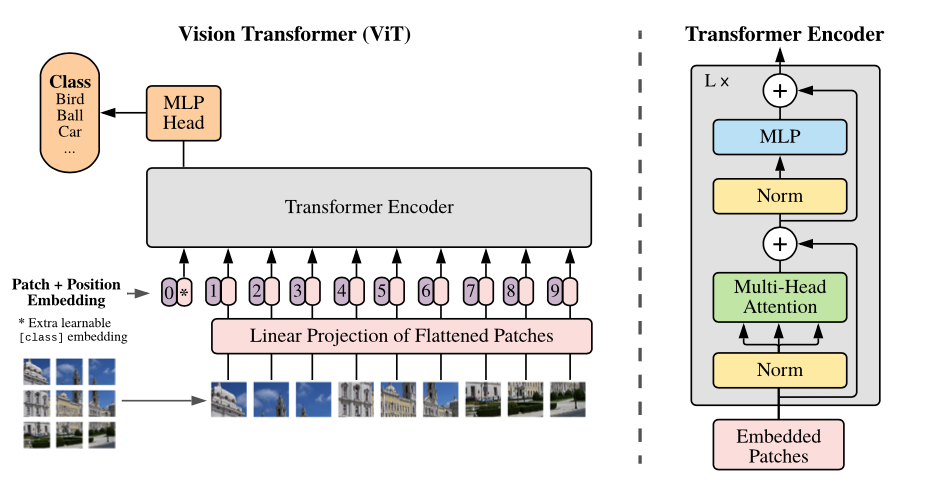
\includegraphics[scale=0.4]{figures/vit_overall.png}
\caption{ViTのアーキテクチャ全体図. 文献\cite{ViT}より引用. (C) 2021 ICLR \label{fig:vit_overall}}
\end{figure}

\newpage
\section{Restormer}
Restormer\cite{Restormer}はTransformerを活用した手法で, ノイズ除去をはじめとした画像復元タスクにおいて高い性能を示す. 図\ref{fig:Restomer_overall}の通りU-Netをベースに作られており, 各層にはTransformer Blockが配置されている. またTransfomer Blockの数は階層が下がるほど増加する. Transformer BlockにはMulti-Dconv head transposed attention (MDTA) とGated-Dconv feed-forward network (GDFN) が含まれており, このうちTransformerを持つMDTAが画像の文脈情報を抽出している. Restormerは, 画像ノイズ除去を含む様々な画像復元タスクにおいて従来手法を上回る優れた性能を示す一方で, 複雑なネットワーク構造をしていることやTransformerを多用していることから学習および推論時の計算コストが大きいことが課題である. 手法の詳細は文献\cite{Restormer}を参照されたい. 

\begin{figure}[htbp]
\centering
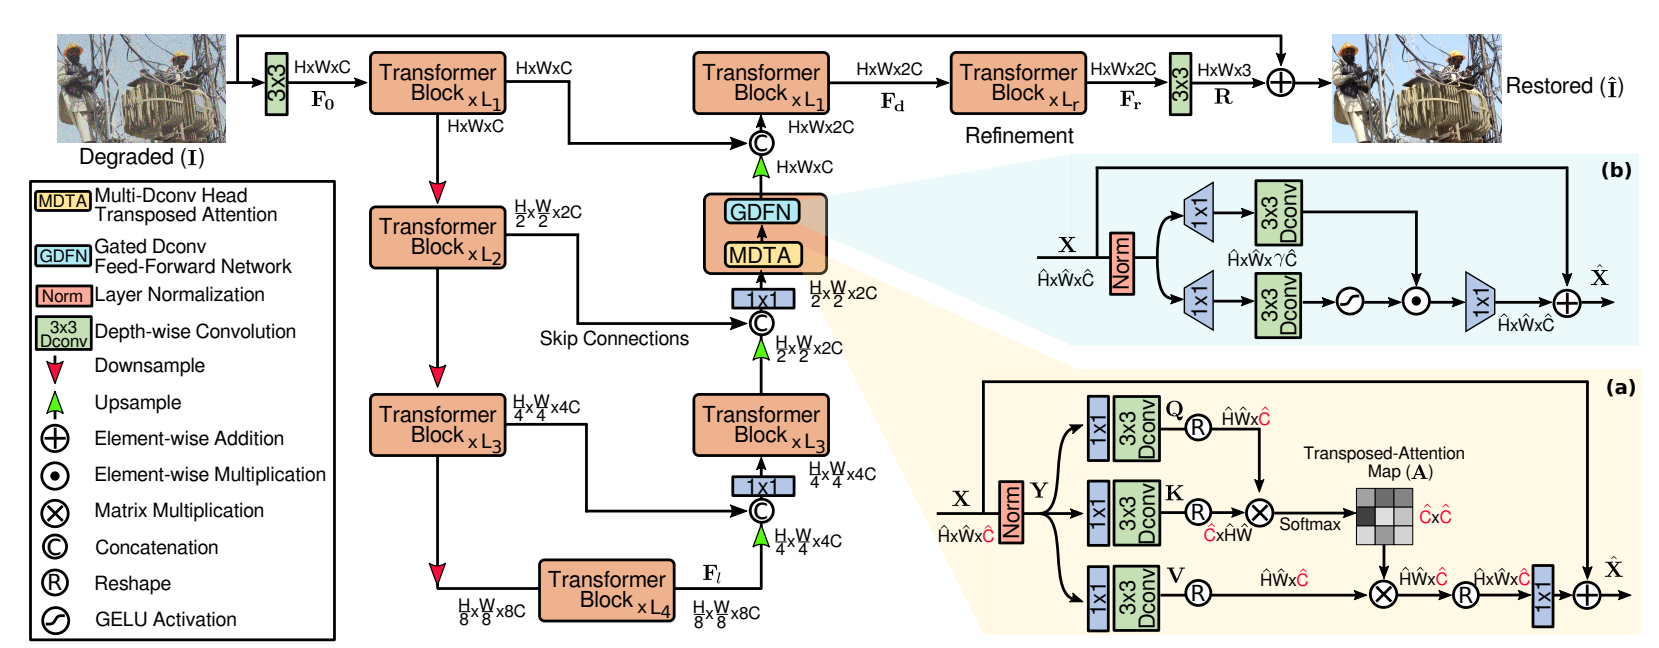
\includegraphics[scale=0.29]{figures/Architecture_of_Restormer.png}
\caption{Restomerのアーキテクチャ全体図. 文献\cite{Restormer}より引用. (C) 2022 IEEE/CVF \label{fig:Restomer_overall}}
\end{figure}

 